\begin{frame}
    \frametitle{
        Numerical Quadrature~(\citeauthor[p.~397]{salgado_classical_2022})
    } % \citetitle[p.~397]{salgado_classical_2022}

    Let
    \begin{math}
        f\in
        \continuous
    \end{math}.
    We seek calculate an approximation of
    \begin{equation*}
        I^{\left(a,b\right)}
        \left[f\right]\coloneqq
        \int_{a}^{b}
        f\left(x\right)
        \dl x.
    \end{equation*}

    Suppose that
    \begin{math}
        g\in
        \continuous
    \end{math},
    whose antiderivative is simply obtained, and
    \begin{math}
        {\left\|f-g\right\|}_{\infty}<
        \varepsilon
    \end{math}.
    Then,
    \begin{equation*}
        \left|
        \int_{a}^{b}
        f\left(x\right)
        \dl x-
        \int\limits_{a}^{b}
        g\left(x\right)
        \dl x
        \right|\leq
        \varepsilon
        \left(b-a\right).
    \end{equation*}

    \begin{definition}[Nodal set]
        Let
        \begin{math}
            \interval\subset
            \mathbb{R}
        \end{math}.
        $X$ is called a \emph{nodal set} of size $n+1\in\mathbb{N}$
        iff
        \begin{math}
            \nodalset\subset
            \interval
        \end{math}
        is a set of distinct elements.
        The elements of $X$, $x_{i}$ are called \emph{nodes}.
    \end{definition}

    \begin{definition}[Interpolating polynomial]
        Suppose that
        \begin{math}
            \nodalset\subset
            \interval
        \end{math}
        is a nodal set and
        \begin{math}
            f\colon
            \interval\to
            \mathbb{R}
        \end{math}
        is a function.
        The function
        \begin{math}
            I\colon
            \interval\to
            \mathbb{R}
        \end{math}
        is called an \emph{interpolant of} $f$ subordinate to $X$ iff
        \begin{math}
            \forall i=0,\dotsc,n:
            I\left(x_{i}\right)=
            f\left(x_{i}\right)
        \end{math},
        we write
        \begin{math}
            I\left(X\right)=
            f\left(X\right)
        \end{math}.
    \end{definition}
\end{frame}

\begin{frame}
    % TODO: Interpolant
    % \begin{definition}[Interpolant]
    %     Suppose
    %     \begin{math}
    %         Y=
    %         {\left\{y_{i}\right\}}_{i=0}^{n}\subset
    %         \mathbb{R}
    %     \end{math}
    %     is a set of not necessarily distinct points.
    %     Define the set of ordered pairs
    %     \begin{equation*}
    %         O=
    %         \left\{
    %         \left(x_{i},y_{i}\right)\mid
    %         x_{i}\in X,
    %         y_{i}\in Y,
    %         \forall i=0,\dotsc,n
    %         \right\}.
    %     \end{equation*}
    %     We say that $I$ is an \emph{interpolant} of $O$ iff
    %     \begin{math}
    %         \forall i=0,\dotsc,n:
    %         I\left(x_{i}\right)=
    %         y_{i}
    %     \end{math},
    %     we write
    %     \begin{math}
    %         I\left(X\right)=
    %         Y
    %     \end{math}.
    %     If the interpolant $I$ is a polynomial, it is called an
    %     \emph{interpolating polynomial}.
    % \end{definition}

    \begin{theorem}[existence and uniqueness]
        Suppose that
        \begin{math}
            \nodalset\subset
            \interval
        \end{math}
        is a nodal set
        and
        \begin{math}
            Y=
            {\left\{
            y_{i}
            \right\}}_{i=0}^{n}\subset
            \mathbb{R}
        \end{math}.
        There is a unique polynomial $p\in\mathbb{P}_{n}$ with the
        property that $p\left(X\right)=Y$.
    \end{theorem}

    % TODO: Interpolation operator
    % \begin{definition}[Interpolation operator]
    %     Suppose that
    %     \begin{math}
    %         \nodalset\subset
    %         \interval
    %     \end{math}.
    %     The \emph{interpolation operation} subordinate to $X$,
    %     denoted
    %     \begin{equation*}
    %         \mathcal{I}_{X}\colon
    %         \continuous\to
    %         \mathbb{P}_{n},
    %     \end{equation*}
    %     is defined as follows: for
    %     \begin{math}
    %         f\in
    %         \continuous
    %     \end{math},
    %     \begin{math}
    %         \mathcal{I}_{X}
    %         \left[f\right]\in
    %         \mathbb{P}_{n}
    %     \end{math}
    %     is the unique interpolating polynomial satisfying
    %     \begin{math}
    %         \mathcal{I}_{X}
    %         \left[f\right]
    %         \left(X\right)=
    %         f\left(X\right)
    %     \end{math}.
    % \end{definition}

    \begin{definition}[Lagrange nodal basis]
        Suppose that
        \begin{math}
            \nodalset\subset
            \interval
        \end{math}
        is a nodal set.
        The \emph{Lagrange nodal basis} subordinate to $X$ is the set
        of polynomials
        \begin{math}
            \mathcal{L}_{X}=
            {\left\{
            L_{\ell}
            \right\}}_{\ell=0}^{n}\subset
            \mathbb{P}_{n}
        \end{math}
        defined via
        \begin{equation*}
            L_{\ell}
            \left(x\right)=
            \prod\limits_{\substack{i=0\\i\neq\ell}}^{n}
            \dfrac{x-x_{i}}{x_{\ell}-x_{i}}.
        \end{equation*}
    \end{definition}

    % TODO: Properties of \mathcal{L}_{X}

    % TODO: interpolating polynomial

    \begin{definition}[Lagrange interpolating polynomial]
        Suppose that
        \begin{math}
            \nodalset\subset
            \interval
        \end{math}
        is a nodal set,
        \begin{math}
            \mathcal{L}_{X}=
            {\left\{L_{i}\right\}}_{i=0}^{n}
            \subset
            \mathbb{P}_{n}
        \end{math}
        is the Lagrange nodal basis subordinate to $X$, and
        \begin{math}
            f\colon
            \interval\to
            \mathbb{R}
        \end{math}.
        The \emph{Lagrange interpolating polynomial} of the function
        $f$, subordinate to the nodal set $X$, is the polynomial
        \begin{equation*}
            p\left(x\right)=
            \sum_{i=0}^{n}
            f\left(x_{i}\right)
            L_{i}\left(x\right)\in
            \mathbb{P}_{n}.
        \end{equation*}
    \end{definition}
\end{frame}

\begin{frame}
    Suppose that
    \begin{math}
        \nodalset\subset
        \interval
    \end{math}
    is a nodal set and $p\in\mathbb{P}_{n}$ is the unique Lagrange
    interpolating polynomial of $f$ subordinate to $X$.
    Then
    \begin{equation*}
        \forall i=0,\dotsc,n:
        f\left(x_{i}\right)=
        p\left(x_{i}\right)
    \end{equation*}
    and
    \begin{equation*}
        \forall x\in
        \interval:
        f\left(x\right)=
        p\left(x\right)+
        E\left(x\right),
    \end{equation*}
    where $E$ is an expression of the interpolation error.
    Then
    \begin{equation*}
        \int_{a}^{b}
        f\left(x\right)
        \dl x=
        \int_{a}^{b}
        p\left(x\right)
        \dl x+
        \int_{a}^{b}
        E\left(x\right)
        \dl x.
    \end{equation*}
    But
    \begin{equation*}
        \int_{a}^{b}
        p\left(x\right)
        \dl x=
        \int_{a}^{b}
        \sum_{i=0}^{n}
        f\left(x_{i}\right)
        L_{i}\left(x\right)=
        \sum_{i=0}^{n}
        f\left(x_{i}\right)
        \int_{a}^{b}
        L_{i}\left(x\right)=
        \sum_{i=0}^{n}
        f\left(x_{i}\right)
        \beta_{i},
    \end{equation*}
    where $L_{i}\in\mathbb{P}_{n}$ is the $i$th Lagrange nodal basis
    element and $\beta_{i}$ is its definite integral:
    \begin{equation*}
        \beta_{i}=
        \int_{a}^{b}
        L_{i}\left(x\right)
        \dl x.
    \end{equation*}
    The expression
    \begin{math}
        \sum_{i=0}^{n}
        f\left(x_{i}\right)
        \beta_{i}
    \end{math}
    is a typical numerical integration formula
    \begin{equation*}
        \left|
        \int_{a}^{b}
        f\left(x\right)
        \dl x-
        \sum_{i=0}^{n}
        f\left(x_{i}\right)
        \beta_{i}
        \right|=
        \left|
        \int_{a}^{b}
        E\left(x\right)
        \dl x
        \right|\leq
        \int_{a}^{b}
        \left|
        E\left(x\right)
        \right|
        \dl x.
    \end{equation*}
\end{frame}

\begin{frame}
    The \emph{quadrature weights}, $\beta_{i}$, depends only on the
    positions of the nodes within $\interval$, as well as the
    interval $\interval$ itself.
    % Suppose that $n=1$, $x_{0}=a$ and $x_{1}=b$.
    % Then
    % \begin{equation*}
    %     p\left(x\right)=
    %     f\left(a\right)
    %     \dfrac{x-b}{a-b}+
    %     f\left(b\right)
    %     \dfrac{x-a}{b-a}
    % \end{equation*}
    % and
    % \begin{equation*}
    %     \int_{a}^{b}
    %     p\left(x\right)
    %     \dl x=
    %     \dfrac{f\left(a\right)}{a-b}
    %     \int_{a}^{b}
    %     \left(x-b\right)
    %     \dl x+
    %     \dfrac{f\left(b\right)}{b-a}
    %     \int_{a}^{b}
    %     \left(x-a\right)
    %     \dl x=
    %     \dfrac{b-a}{2}
    %     \left(f\left(a\right)+f\left(b\right)\right).
    % \end{equation*}
    We will consider the approximation of a weight integral
    \begin{equation*}
        I^{\left(a,b\right)}_{w}
        \left[f\right]\coloneqq
        \int_{a}^{b}
        f\left(x\right)
        w\left(x\right)
        \dl x.
    \end{equation*}

    \begin{definition}[Quadrature rule]
        Suppose that $n,r\in\mathbb{N}_{0}$,
        $w$ is a weight function on
        \begin{math}
            \interval\subset
            \mathbb{R}
        \end{math},
        $h=b-a>0$, and
        \begin{math}
            f\in
            C^{r}\left(
            \interval
            \right)
        \end{math}.
        The expression
        \begin{equation*}
            Q^{\left(a,b\right)}_{w,r}
            \left[f\right]=
            \sum_{i=0}^{r}
            \sum_{j=0}^{n}
            \beta_{i,j}
            f^{\left(i\right)}
            \left(x_{j}\right)=
            \sum_{j=0}^{n}
            \left(
            \beta_{0,j}
            f\left(x_{j}\right)+
            \beta_{1,j}
            f^{\prime}
            \left(x_{j}\right)+
            \cdots+
            \beta_{r,j}
            f^{\left(r\right)}
            \left(x_{j}\right)
            \right),
        \end{equation*}
        where
        \begin{equation*}
            \forall i\in
            \left\{0,\dotsc,r\right\}:
            \forall j\in
            \left\{0,\dotsc,n\right\}:
            \beta_{i,j}=
            h^{i+1}
            \widehat{\beta}_{i,j}
        \end{equation*}
        and
        \begin{equation*}
            \forall j\in
            \left\{0,\dotsc,n\right\}:
            x_{j}=
            a+
            h\cdot
            \widehat{x}_{j},
        \end{equation*}
        is called a \emph{quadrature rule of degree $r$} with
        \emph{intrinsic nodes}
        \begin{math}
            \widehat{X}=
            \left\{
            \widehat{x}_{j}
            \right\}\subset
            \left[0,1\right]
        \end{math}
        and \emph{intrinsic weights}
        \begin{math}
            \left\{
            \beta_{i,j}
            \right\}
            \subset
            \mathbb{R}
        \end{math}
        are called the \emph{effective nodes} and
        \emph{effective weights}, respectively.
    \end{definition}
    A quadrature rule of degree $r=0$ is called a
    \emph{simple quadrature rule}, and we simplify the notation
    by writing $\beta_{j}=\beta_{0,j}$ and
    \begin{equation*}
        Q^{\left(a,b\right)}_{w,r}
        \left[f\right]=
        \sum_{j=0}^{n}
        \beta_{j}
        f^{\left(i\right)}
        \left(x_{j}\right).
    \end{equation*}
\end{frame}

\begin{frame}

    The \emph{quadrature rule error} is defined as
    \begin{equation*}
        E_{Q}
        \left[f\right]=
        I^{\left(a,b\right)}_{w}
        \left[f\right]-
        Q^{\left(a,b\right)}_{w,r}
        \left[f\right].
    \end{equation*}

    \begin{definition}[consistency]
        The quadrature rule is \emph{consistent of order at least}
        $m\in\mathbb{N}_{0}$ iff $E_{Q}\left[q\right]=0$ for all
        $q\in\mathbb{P}_{m}$.
        The quadrature rule is \emph{consistent of order exactly} $m$
        iff $E_{Q}\left[q\right]=0$ for all $q\in\mathbb{P}_{m}$;
        however, for some $r\in\mathbb{P}_{m+1}$,
        $E_{Q}\left[r\right]\neq 0$.
    \end{definition}

    \begin{definition}[interpolatory quadrature rule]
        Assume that $n\in\mathbb{N}_{0}$, $w$ is a weight function on
        $\interval\subset\mathbb{R}$, and $f\in\continuous$.
        Suppose that $\nodalset\subset\interval$ is a nodal set and
        $p\in\mathbb{P}_{n}$ is the unique Lagrange Interpolating
        polynomial of $f$ subordinate to $X$, with
        \begin{equation*}
            p\left(x\right)=
            \sum_{j=0}^{n}
            f\left(x_{j}\right)
            L_{j}\left(x\right),
        \end{equation*}
        where $L_{j}\in\mathbb{P}_{n}$ is the $j$th Lagrange nodal
        basis element.
    \end{definition}
    The expression
    \begin{equation*}
        Q^{\left(a,b\right)}_{w}
        \left[f\right]=
        \sum_{j=0}^{n}
        f\left(x_{j}\right)
        \beta_{j},
    \end{equation*}
    where
    \begin{equation*}
        \beta_{j}=
        \int_{a}^{b}
        L_{j}\left(x\right)
        w\left(x\right)
        \dl x,
    \end{equation*}
    is called an \emph{interpolatory quadrature rule subordinate to $X$ of Lagrange type}
    for approximating
    \begin{math}
        I^{\left(a,b\right)}_{w}
        \left[f\right]
    \end{math}.
    % TODO: Hermite
    % Suppose that $f\in $
\end{frame}

\begin{frame}
    \begin{theorem}[existence and uniqueness]
        Suppose that $\nodalset\subset\mathbb{R}$ is a nodal set.
        There exists uniqueness weights $\left\{\beta_{j}\right\}_{j=0}^{n}$
        such that
        \begin{equation*}
            \forall q\in\mathbb{P}_{n}:
            \int_{a}^{b}
            q\left(x\right)
            w\left(x\right)
            \dl x=
            \sum_{j=0}^{n}
            \beta_{j}
            q\left(x_{j}\right),
        \end{equation*}
        or, equivalently,
        \begin{equation*}
            \forall q\in\mathbb{P}_{n}:
            E_{Q}\left[q\right]=0.
        \end{equation*}
        Moreover, these weights are given by
        \begin{equation*}
            \forall j\in\left\{0,\dotsc,n\right\}:
            \beta_{j}=
            \int_{a}^{b}
            L_{j}\left(x\right)
            w\left(x\right)
            \dl x,
        \end{equation*}
        where $L_{j}$ is the $j$th Lagrange nodal basis polynomial subject to $X$.
    \end{theorem}

    % TODO: Remark
    \begin{theorem}[consistency]
        The last result shows that the simple quadrature rule,
        \begin{equation*}
            Q^{\left(a,b\right)}_{w}
            \left[f\right]=
            \sum_{j=0}^{n}
            \beta_{i}
            f\left(x_{i}\right),
        \end{equation*}
        is consistent of order at least $n$ iff it is a quadrature
        rule of Lagrange type.
    \end{theorem}
\end{frame}

\begin{frame}
    \begin{theorem}[Error estimate]
        Suppose that $n\in\mathbb{N}_{0}$, $w$ is a weight function
        on
        \begin{math}
            \interval\subset
            \mathbb{R}
        \end{math}.
        \begin{math}
            f\in C^{n+1}
            \left(
            \interval
            \right)
        \end{math},
        and
        \begin{math}
            X=
            \left\{x_{i}\right\}_{i=0}^{n}\subset
            \interval
        \end{math}
        is a nodal set.
        Suppose that
        \begin{math}
            Q^{\left(a,b\right)}_{w}
            \left[f\right]
        \end{math}
        is the interpolatory quadrature rule subordinate to $X$ of Lagrange type.
        Then,
        \begin{equation*}
            \left|
            E_{Q}
            \left[f\right]
            \right|\leq
            \dfrac{M_{n+1}}{\left(n+1\right)!}
            \int_{a}^{b}
            \left|
            \omega_{n+1}
            \left(x\right)
            \right|
            w\left(x\right)
            \dl x,
        \end{equation*}
        where
        \begin{equation*}
            \omega_{n+1}
            \left(x\right)=
            \prod\limits_{j=0}^{n}
            \left(x-x_{j}\right)
        \end{equation*}
        and
        \begin{equation*}
            M_{n+1}=
            {\left\|
            f^{\left(n+1\right)}
            \right\|}_{\infty}.
        \end{equation*}
        Consequently, an interpolatory quadrature rule subordinate to
        $X$ of Lagrange type is consistent of order at least $n$.
    \end{theorem}
    % Error hermite
    % \begin{theorem}[error estimate]
    %     Suppose that $n\in\mathbb{N}_{0}$, $w$ is a weight function on
    %     $\interval\subset\mathbb{R}$, $f\in C^{\left(2n+2\right)}\left(\interval\right)$,
    %     and $\nodalset\subset\interval$ is a nodal set.
    %     Suppose that
    %     \begin{math}
    %         Q^{\left(a,b\right)}_{w,1}
    %         \left[f\right]    
    %     \end{math}
    %     is the interpolatory quadrature rule subordinate to $X$
    % \end{theorem}
    \begin{definition}[characteristic function]
        Suppose that $B\subset\mathbb{R}$.
        The \emph{characteristic function} of $B$ is the function
        \begin{equation*}
            \chi_{B}\left(t\right)=
            \begin{cases}
                1, & t\in B,                    \\
                0, & t\in\mathbb{R}\setminus B.
            \end{cases}
        \end{equation*}
    \end{definition}
\end{frame}

\begin{frame}
    % TODO: lemma
    \begin{theorem}[kernel]
        Suppose that $r\in\mathbb{N}_{0}$ and $m\in\mathbb{N}$, with
        $m>r$.
        Define the function
        \begin{math}
            k_{m}\colon
            \interval\times\interval\to
            \mathbb{R}
        \end{math}
        via
        \begin{equation*}
            k_{m}\left(x,y\right)=
                {\left(x-y\right)}^{m}
            \xi_{\left[a,x\right]}\left(y\right)=
            \begin{cases}
                \left(x-y\right)^{m}, & a\leq y\leq x\leq b, \\
                0,                    & a\leq x< y\leq b.
            \end{cases}
        \end{equation*}
        Then, for each $i\in\left\{0,\dotsc,r\right\}$,
        \begin{equation*}
            \diffp[i]{k_{m}}{x}\in
            C\left(\interval\times\interval\right)
        \end{equation*}
        and
        \begin{equation*}
            \diffp[i]{k_{m}\left(x,y\right)}{x}=
            \begin{cases}
                \prod\limits_{k=0}^{i-1}
                \left(m-k\right)
                {\left(x-y\right)}^{m-i}, & a\leq y\leq x\leq b, \\
                0,                        & a\leq x< y\leq b.
            \end{cases}
        \end{equation*}
    \end{theorem}
\end{frame}

\begin{frame}
    \begin{theorem}[Peano Kernel Theorem]
        Suppose that $r\in\mathbb{N}_{0}$, $m\in\mathbb{N}$, with $m>n$,
        $w$ is a weight function on $\left[a,b\right]\subset\mathbb{R}$, and
        $f\in C^{m+1}\left(\interval\right)$.
        Assume that
        \begin{math}
            Q^{\left(a,b\right)}_{w,r}
            \left[f\right]
        \end{math}
        is a quadrature rule of degree $r$,
        that is consistent of order at least $m$.
        Let the function
        \begin{math}
            k_{m}\colon\interval\times\interval\to\mathbb{R}
        \end{math}.
        Set
        \begin{equation*}
            K_{m}\left(y\right)=
            E_{Q}\left[k_{m}\left(\cdot, y\right)\right]=
            \int_{a}^{b}
            k_{m}\left(x,y\right)w\left(x\right)\dl x-
            \sum_{j=0}^{n}
            \sum_{i=0}^{r}
            \beta_{i,j}
            \diffp[i]{k_{m}\left(x_{j},y\right)}{x}.
        \end{equation*}
        Then the quadrature error satisfies
        \begin{equation*}
            E_{Q}\left[f\right]=
            \dfrac{1}{m!}
            \int_{a}^{b}
            f^{\left(m+1\right)}\left(y\right)
            K_{m}\left(y\right)
            \dl y.
        \end{equation*}
        The function $K_{m}\left(y\right)$ is called the \emph{Peano Kernel}.
    \end{theorem}

    % TODO: remark
    % \begin{theorem}[Peano Kernel]
    %     Re.
    % \end{theorem}
    \begin{theorem}[quadrature error stability]
        We have
        \begin{equation*}
            \left|
            E_{Q}
            \left[f\right]
            \right|\leq
            \dfrac{1}{m!}
            {\left\|
                f^{\left(m+1\right)}
                \right\|}_{\infty}
            {\left\|
                K_{m}
                \right\|}_{1}.
        \end{equation*}
        Since ${\left\|K_{m}\right\|}_{1}<\infty$, there is a
        constant $C>0$ that may depend on the size of the interval
        but is independent of $f$ such that
        \begin{equation*}
            \left|
            E_{Q}
            \left[f\right]
            \right|\leq
            C{\left\|
                    f^{\left(m+1\right)}
                    \right\|}_{\infty}.
        \end{equation*}
    \end{theorem}
\end{frame}

\begin{frame}
    % TODO: Theorem
    \begin{theorem}[constant sign]
        If $K_{m}$ does not change sign in $\interval$, then
        \begin{equation*}
            E_{Q}\left[f\right]=
            \dfrac{f^{\left(m+1\right)\left(\xi\right)}}{m!}
            \int_{a}^{b}K_{m}
            \dl y
        \end{equation*}
        for some $\xi\in\interval$.
        Furthermore, we have the simple representation for the error
        \begin{equation*}
            E_{Q}\left[f\right]=
            \dfrac{E_{Q}\left[x^{m+1}\right]}{\left(m+1\right)!}
            f^{\left(m+1\right)}\left(\xi\right)
        \end{equation*}
        for some $\xi\in\interval$, where $E_{Q}\left[x^{m+1}\right]$
        is the quadrature error for the function $x\mapsto x^{m+1}$.
    \end{theorem}

    \begin{definition}[Peano Kernel]
        Let $M_{1}=\chi_{\interval}$.
        For $k\in\mathbb{N}$ with $k\geq 2$, set
        \begin{equation*}
            M_{k}\left(x\right)=
            \int_{\mathbb{R}}
            M_{k-1}\left(x-y\right)M_{1}\left(y\right)
            \dl y.
        \end{equation*}
        For $k\in\mathbb{N}$ and $h>0$, we define
        \begin{equation*}
            M_{k}\left(x,h\right)=
            \dfrac{1}{h}
            M_{k}
            \left(\dfrac{x}{h}\right).
        \end{equation*}
    \end{definition}
    % TODO: lemma
    % TODO: integral representation
    % TODO: modulus of smoothness
    % TODO: scaling argument
\end{frame}

\begin{frame}
    \begin{definition}[Closed Newton-Cotes quadrature rule]
        Suppose that $w$ is a weight function on
        \begin{math}
            \interval\subset
            \mathbb{R}
        \end{math}
        and $n\in\mathbb{N}$.
        Set $h=b-a>0$ and $\hslash=\frac{h}{n}$.
        Suppose that, for the simple quadrature rule, the nodal set
        $\nodalset\subset\interval$ is defined by
        \begin{equation*}
            x_{j}=
            a+j\hslash,\quad
            j\in\left\{0,\dotsc,n\right\}.
        \end{equation*}
        The resulting method, denoting $Q_{n}\left[f\right]$, is
        called a \emph{closed Newton-Cotes quadrature rule of order $n$}.
    \end{definition}

    \begin{example}[Newton-Cotes quadrature rules of order $n=1,2$ and weight function $w\equiv 1$ on $\interval$]
        \begin{equation*}
            x_{j}=
            a+h\widehat{x}_{j},\quad
            \beta_{j}=h\widehat{\beta}_{j},\quad
            h=b-a.
        \end{equation*}

        \begin{table}[ht!]
            \centering
            \begin{tabular}{ccccc}
                \hline
                $n$ & rule                                                         & $\widehat{x}_{j}$ & $\widehat{\beta}_{j}$
                    & Error Formula                                                                                                              \\
                $1$ & Trapezoidal                                                  & $0,1$             & $\frac{1}{2}, \frac{1}{2}$
                    & $-\frac{1}{12}\hslash^{3}f^{\left(2\right)}\left(\xi\right)$                                                               \\
                $2$ & Simpson's                                                    & $0,\frac{1}{2},1$ & $\frac{1}{6}, \frac{4}{6}, \frac{1}{6}$
                    & $-\frac{1}{90}\hslash^{5}f^{\left(4\right)}\left(\xi\right)$                                                               \\
                \hline
            \end{tabular}
        \end{table}
        For $n=2$, we observe the phenomenon of
        \alert{super-convergence}, i.e., a higher than expected convergence.

        For example, consider the case $n=3$, Simpson's $\frac{3}{8}$
        rule, on the reference interval $\left[0,1\right]$.
        The second Lagrange nodal basis element is
        \begin{equation*}
            \widehat{L}_{1}\left(x\right)=
            \dfrac{
                x
                \left(x-\frac{2}{3}\right)
                \left(x-1\right)
            }{
                \frac{1}{3}
                \left(\frac{1}{3}-\frac{2}{3}\right)
                \left(\frac{1}{3}-1\right)
            }=
            \dfrac{27}{2}
            \left(
            x^{3}-\dfrac{5}{3}x^{2}+\dfrac{2}{3}x
            \right).
        \end{equation*}
        Then,
        \begin{equation*}
            \widehat{\beta}_{1}=
            \int_{0}^{1}
            \widehat{L}_{1}\left(x\right)
            \dl x=
            \dfrac{27}{2}
            {\left.
                \left(
                \dfrac{1}{4}x^{4}-
                \dfrac{5}{9}x^{3}+
                \dfrac{1}{3}x^{2}
                \right)
                \right|}_{x=0}^{x=1}=
            \dfrac{3}{8}.
        \end{equation*}
    \end{example}
\end{frame}

\begin{frame}
    \begin{theorem}[Error estimate]
        Let
        \begin{math}
            \interval\subset
            \mathbb{R}
        \end{math}.
        Suppose that $Q^{\left(a,b\right)}_{n}\left[f\right]$ is a
        closed Newton-Cotes quadrature rule of order
        $n\in\mathbb{N}$.
        Then, the order of quadrature rule is consistent of order at
        least $n$.
        Moreover, if $f\in C^{n+1}\left(\interval\right)$, then
        \begin{equation*}
            \left|
            E_{Q_{n}}
            \left[f\right]
            \right|\leq
            C
            h^{n+2}
            {\left\|f^{\left(n+1\right)}\right\|}_{\infty},
        \end{equation*}
        where $h=b-a$ and $C>0$ is independent of $h$ and $f$.
    \end{theorem}

    \begin{theorem}[Integral Mean Value Theorem]
        Suppose that
        \begin{math}
            -\infty<a<b<\infty
        \end{math},
        \begin{math}
            f\in
            \continuous
        \end{math},
        and
        \begin{math}
            g\in
            \mathcal{R}
            \left(a,b\right)
        \end{math}.
        Furthermore, suppose that
        \begin{math}
            \forall x\in\interval:
            g\left(x\right)\geq0
        \end{math}.
        Then there exists a point $\xi\in\interval$ such that
        \begin{equation*}
            \int_{a}^{b}
            f\left(x\right)
            g\left(x\right)
            \dl x=
            f\left(\xi\right)
            \int_{a}^{b}
            g\left(x\right)
            \dl x.
        \end{equation*}

        Thus, if
        \begin{math}
            \forall x\in
            \interval:
            g\left(x\right)=
            1
        \end{math},
        there exists a point $\xi\in\interval$ such that
        \begin{equation*}
            f\left(\xi\right)=
            \dfrac{1}{b-a}
            \int_{a}^{b}
            f\left(x\right)
            \dl x.
        \end{equation*}
    \end{theorem}
\end{frame}

\section{Heuristic derivation of Advection Differential Equation}

\begin{frame}
    \begin{definition}[Average concentration]
        Let $h>0$, $h\ll 1$.
        We define the \emph{average concentration}
        $\overline{u}\left(x,t\right)$ in a space-time cell
        \begin{math}
            \left[
                x-\frac{1}{2}h,
                +x\frac{1}{2}h
                \right]\times
            \left[0,T\right]
        \end{math}.

        \begin{equation*}
            \overline{u}
            \left(x,t\right)=
            \dfrac{1}{h}
            \int_{x-\frac{1}{2}h}^{x+\frac{1}{2}h}
            u\left(s,t\right)
            \dl s.
        \end{equation*}
    \end{definition}

    \begin{definition}[Mass flux]
        The mass flux is the product of
        \begin{equation*}
            J_{x}=
            c
            v_{x}.
        \end{equation*}
        \begin{itemize}
            \item

                  $J_{x}$ is the mass flux in $x$-direction.

            \item

                  $c$ is the concentration of the substance.

            \item

                  $v_{x}$ is the velocity of the substance in the
                  $x$-direction.
        \end{itemize}
    \end{definition}

    \begin{theorem}[Conservation law]
        If the species is carried along by a flowing medium with
        velocity $a\left(x,t\right)$, then the mass conservation law
        implies that the change of $\overline{u}\left(x,t\right)$ per
        unit of time is the net balance of inflow and outflow over
        the cell boundaries,
        \begin{equation*}
            \diffp{\overline{u}\left(x,t\right)}{t}=
            \dfrac{1}{h}
            \left[
                a\left(x-\frac{1}{2}h,t\right)
                u\left(x-\frac{1}{2}h,t\right)-
                a\left(x+\frac{1}{2}h,t\right)
                u\left(x+\frac{1}{2}h,t\right)
                \right].
        \end{equation*}
    \end{theorem}
\end{frame}

\begin{frame}
    \frametitle{Numerical Quadrature~(\citeauthor[p.~9]{Hundsdorfer2003})}

    \begin{definition}[Advection equation]
        \begin{equation*}
            \diffp{u\left(x,t\right)}{t}+
            \diffp{a\left(x,t\right)u\left(x,t\right)}{x}=
            0.
            % u_{t}+du_{x}=0.
        \end{equation*}
    \end{definition}

    \begin{definition}[Diffusion equation]
        \begin{equation*}
            \diffp{u\left(x,t\right)}{t}=
            \diffp{}{x}
            \left(
            d\left(x,t\right)\diffp{u\left(x,t\right)}{x}
            \right).
            % u_{t}=du_{xx}.
        \end{equation*}
    \end{definition}

    \begin{figure}[ht!]
        \centering
        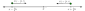
\includegraphics[width=.6\paperwidth]{deduction}
    \end{figure}
\end{frame}

\begin{frame}

    \begin{theorem}[Mass conservation law]
        If $u\left(x,t\right)$ is a concentration and
        \begin{equation*}
            M\left(t\right)\coloneqq
            \int_{0}^{1}
            u\left(x,t\right)
            \dl x
        \end{equation*}
        represents the mass in $\left[0,1\right]$ at time $t$, then
        $M$ is a conserved quantity.
    \end{theorem}

    \begin{proof}
        \begin{align*}
            \diff{M\left(t\right)}{t} & =
            \int_{0}^{1}
            u_{t}\left(x,t\right)
            \dl x=
            \int_{0}^{1}
            \left(
            -au_{x}\left(x,t\right)+
            du_{xx}\left(x,t\right)
            \right)\dl x                  \\
                                      & =
            -a\left(
            u\left(1,t\right)-
            u\left(0,t\right)
            \right)+
            d\left(
            u_{x}\left(1,t\right)-
            u_{x}\left(0,t\right)
            \right)=0.
        \end{align*}
    \end{proof}
\end{frame}

\section{The Advection Problem in One Dimension}

\begin{frame}
    \begin{definition}[space-time grid]
        Let $d\in\mathbb{N}$, $\Omega=\left(0,1\right)^{d}$, and $T>0$.
        For $K, N\in\mathbb{N}$, we set $\tau=\frac{T}{K}$ and
        $h=\frac{1}{N+1}$.
        We define the \emph{space-time grid domain}
        \begin{equation*}
            \overline{\mathcal{C}}^{\tau}_{h}=
            \overline{\Omega}_{h}\times
            {\left[0,T\right]}_{\tau}=
            \left\{
            \left(\mathbf{x},t_{k}\right)\mid
            \mathbf{x}\in\overline{\Omega}_{h},
            t_{k}=k\tau,
            k\in\left\{0,\dotsc,K\right\}
            \right\},
        \end{equation*}
        where we recall that
        \begin{math}
            \overline{\Omega}_{h}=
            \overline{\Omega}\cap
            \mathbb{Z}^{d}_{h}
        \end{math}.
        We define the \emph{discrete interior} of $\overline{C}^{\tau}_{h}$ to be
        \begin{equation*}
            \mathcal{C}^{\tau}_{h}=\Omega_{h}\times
            \left(0,T\right)_{\tau}.
        \end{equation*}
    \end{definition}

    \begin{definition}[space-time grid functions]
        Let $\mathcal{C}^{\tau}_{h}$ be a space-time grid domain.
        We denote by
        \begin{equation*}
            \mathcal{V}
            \left(
            \overline{\mathcal{C}}^{\tau}_{h}
            \right)=
            \left\{
            v\mid
            \overline{C}^{\tau}_{h}\to\mathbb{R}
            \right\}
        \end{equation*}
        be the space of \emph{space-time grid functions}.
        The spaces
        \begin{equation*}
            \mathcal{V}
            \left(
            \mathcal{C}^{\tau}_{h}
            \right),
            \mathcal{V}
            \left(
            \partial_{L}\mathcal{C}^{\tau}_{h}
            \right)
        \end{equation*}
    \end{definition}
\end{frame}

\begin{frame}
    \begin{definition}[space-time discrete norms]
        Let $d\in\left\{1,2\right\}$, $p\in\left[1,\infty\right]$, and
        $q\in\left[1,\infty\right)$.
        We define the \emph{space-time} norm
        \begin{equation*}
            \left\|
            v
            \right\|_{L^{q}_{\tau}\left(L^{p}_{h}\right)}=
                {\left(\tau
                    \sum_{k=1}^{K}
                    \left\|v^{k}\right\|^{q}_{L^{p}_{h}}
                    \right)}^{\frac{1}{q}}
        \end{equation*}
        and
        \begin{equation*}
            \left\|
            v
            \right\|_{L^{\infty}_{\tau}\left(L^{p}_{h}\right)}=
            \max^{K}_{k=0}
            {\left\|
            v^{k}
            \right\|}_{L^{p}_{h}}
        \end{equation*}
    \end{definition}
\end{frame}

\begin{frame}
    \begin{definition}[Péclet number]
        Consider the simple constant-coefficient advection-diffusion
        equation
        \begin{equation*}
            u_{t}+
            au_{x}=
            du_{xx},\quad
            t>0,\quad
            0<x<L,
        \end{equation*}
        with the given initial profile $u\left(x,0\right)$.
        If $d>0$ we need boundary conditions at $x=0$ and $x=L$,
        such as Dirichlet conditions.
        On the other hand, for the pure advection problem we need
        only to prescribe the solution at the \emph{inflow} boundary,
        that is, at $x=0$ if $a>0$ and $x=L$ if $a<0$.
        If $d>0$ but $d\approx0$, or more precisely if the
        \emph{Péclet number}
        \begin{equation*}
            \left|a\right|\frac{L}{d}
        \end{equation*}
        is large, the Dirichlet condition at the outflow boundary
        will give rise to a \emph{boundary layer}.

        If the Péclet number $\left|a\frac{L}{d}\right|$ is large,
        the problem is called \emph{singularity perturbed}.
        % It is assumed that $d>0$, excluding the pure advection case.
        % where $L$ is the length of the spatial interval.
    \end{definition}
\end{frame}